\subsection{Three Dimensional Plot Types}
\label{sec:3d}
\PGFPlots\ provides three dimensional visualizations like scatter, line, mesh or surface plots. This section explains the methods to provide input coordinates and how to use the different plot types.

\subsubsection{Before You Start With 3D}
\label{pgfplots:3d:preliminary}
Before we delve into the capabilities of \PGFPlots\ for three dimensional visualization, let me start with some preliminary remarks. The reason to use \PGFPlots\ for three dimensional plots are similar to those of normal, two dimensional plots: the possibility to get consistent fonts and document consistent styles combined with high--quality output.

While this works very nice for (not too complex) two dimensional plots, it requires considerably more effort than non--graphical documents. This is even more so for three dimensional plots. In other words: \PGFPlots' three dimensional routines are slow. There are reasons for this and some of them may vanish in future versions. But one of these reasons is, that \TeX\ has never been designed for complex visualisation techniques. Consider the image externalization routines mentioned in section~\ref{sec:pgfplots:export}, in particular the |external| library to reduce typesetting time. Besides the speed limitations, three dimensional plots reach memory limits easily. Therefor, the plot complexity of three dimensional plots is limited to relatively coarse resolutions. Section~\ref{sec:pgfplots:export} also discusses methods to extend the initial \TeX\ memory limits.

Another issue which arises in three dimensional visualization is depth. \PGFPlots\ supports $z$ buffering techniques up to a certain extend. It works pretty well for single scatter plots (|z buffer=sort|), mesh or surface plots (|z buffer=auto|) or parametric mesh and surface plots (|z buffer=sort|). However, it can't combine different |\addplot| commands, those will be drawn in the order of appearance.
You may encounter the limitations sometimes. Maybe it will be improved in future versions.

If you decide that you need high complexity, speed and 100\% reliable z buffers (depth information), you should consider using other visualization tools and return to \PGFPlots\ in several years. If you can wait for a complex picture and you don't even see the limitations arising from z buffering limitations, you should use \PGFPlots. Again, consider using the automatic picture externalization with the |external| library discussed in section~\ref{sec:pgfplots:export}.

Enough for now, let's continue.

\subsubsection{The \texttt{\textbackslash addplot3} Command: Three Dimensional Coordinate Input}
\label{pgfplots:sec:threedim}
\begin{addplot3generic}
	The \verbpdfref{\addplot3} command is the main interface for any three dimensional plot. It works in the same way as its two dimensional variant |\addplot| which has been described in all detail in section~\ref{cmd:pgfplots:addplot} on page~\pageref{cmd:pgfplots:addplot}.

	The \verbpdfref{\addplot3} command accepts the same input methods as the |\addplot| variant, including expression plotting, coordinates, files and tables. However, a third coordinate is necessary for each of these methods which is usually straight--forward and is explained in all detail in the following.

	Furthermore, \verbpdfref{\addplot3} has a way to decide whether a \emph{line} visualization or a \emph{mesh} visualization has to be done. The first one is map from one dimension into $\R^3$ and the latter one a map from two dimensions to $\R^3$. Here, the keys |mesh/rows| and |mesh/cols| are used to define mesh sizes (matrix sizes). Usually, you don't have to care about that because the coordinate input routines already allow either one--dimensional or two dimensional structure.
\end{addplot3generic}

\begin{addplot3operation}[]{coordinates}{\marg{coordinate list}}
	The \verbpdfref{\addplot3 coordinates} method works like its two--dimensional variant, \verbpdfref{\addplot coordinates} which is described in all detail on page~\pageref{pgfplots:addplot:coordinates}:

	A long list of coordinates |(|\meta{x}|,|\meta{y}|,|\meta{z}|)| is expected, separated by white spaces. The input list can be either an unordered series of coordinates, for example for scatter or line plots. It can also have matrix structure, in which case an empty input line (which is equivalent to ``|\par|'') marks the end of one matrix row. Matrix structure can also be provided if one of |mesh/rows| or |mesh/cols| is provided explicitly.
	
\long\def\temporarytest{\noexpand\par}
\begin{codeexample}[newline=\temporarytest]
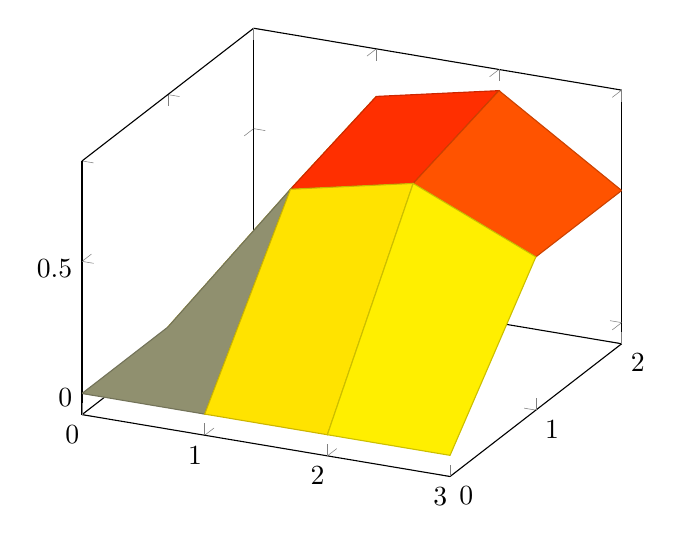
\begin{tikzpicture}
	\begin{axis}
		% this yields a 3x4 matrix:
		\addplot3[surf] coordinates {
			(0,0,0) (1,0,0)   (2,0,0)   (3,0,0)

			(0,1,0) (1,1,0.6) (2,1,0.7) (3,1,0.5)

			(0,2,0) (1,2,0.7) (2,2,0.8) (3,2,0.5)
		};
	\end{axis}
\end{tikzpicture}
\end{codeexample}
	\noindent Here, \verbpdfref{\addplot3} reads a matrix with three rows and four columns. The empty lines separate one row from the following.

	As for the two--dimensional |plot coordinates|, it is possible to provide (constant) mathematical expressions inside of single coordinates. The syntax |(|\meta{x}|,|\meta{y}|,|\meta{z}|) |\oarg{meta} can be used just as for two dimensional |plot coordinates| to provide explicit color data; error bars are also supported.
\end{addplot3operation}

\begin{addplot3operation}[]{file}{\marg{name}}
	The \verbpdfref{\addplot3 file} input method is the same as \verbpdfref{\addplot file} -- it only expects one more coordinate.
	Thus, the input file contains $x_i$ in the first column, $y_i$ in the second column and $z_i$ in the third. 
	
	A further column is read after $z_i$ if |point meta=explicit| has been requested, see the documentation of \verbpdfref{\addplot file} on page~\pageref{pgfplots:addplot:file} for details.
	
	As for \verbpdfref{\addplot3 coordinates}, an empty line in the file marks the end of one matrix row.
\begin{codeexample}[]
\begin{tikzpicture}
	\begin{axis}
		% We have `plotdata/first3d.dat' with
		%---------
		% 0 0 0.8
		% 1 0 0.56
		% 2 0 0.5
		% 3 0 0.75
		%
		% 0 1 0.6
		% 1 1 0.3
		% 2 1 0.21
		% 3 1 0.3
		%
		% 0 2 0.68
		% 1 2 0.22
		% 2 2 0.25
		% 3 2 0.4
		%
		% 0 3 0.7
		% 1 3 0.5
		% 2 3 0.58
		% 3 3 0.9
		% -> yields a 4x4 matrix:
		\addplot3[surf] file {plotdata/first3d.dat};
	\end{axis}
\end{tikzpicture}
\end{codeexample}

	For matrix data in files, it is important to specify the ordering in which the matrix entries have been written. The default configuration is |mesh/ordering=x varies|, so you need to change it to |mesh/ordering=y varies| in case you have columnwise ordering.
\end{addplot3operation}

\begin{addplot3operation}[]{table}{\oarg{column selection}\marg{file}}
	The \verbpdfref{\addplot3 table} input works in the same way as its two dimensional counterpart \verbpdfref{\addplot table}. It only expects a column for the $z$ coordinates. Furthermore, it interprets empty input lines as end--of--row (more generally, end--of--scanline) markers, just as for |plot file|. The remarks above about the |mesh/ordering| applies here as well.
\end{addplot3operation}

\begin{pgfplotskeylist}{mesh/rows=\marg{integer},mesh/cols=\marg{integer}}
	For visualization of mesh or surface plots which need some sort of matrix input, the dimensions of the input matrix need to be known in order to visualize the plots correctly. The matrix structure may be known from end--of--row marks (empty lines as general end--of--scanline markers in the input stream) as has been described above.

	If the matrix structure is not yet known, it is necessary to provide at least one of |mesh/rows| or |mesh/cols| where |mesh/rows| indicates the number of samples for $y$ coordinates whereas |mesh/cols| is the number of samples used for $x$ coordinates (see also |mesh/ordering|). 

	Thus, the following example is also a valid method to define an input matrix.
\begin{codeexample}[]
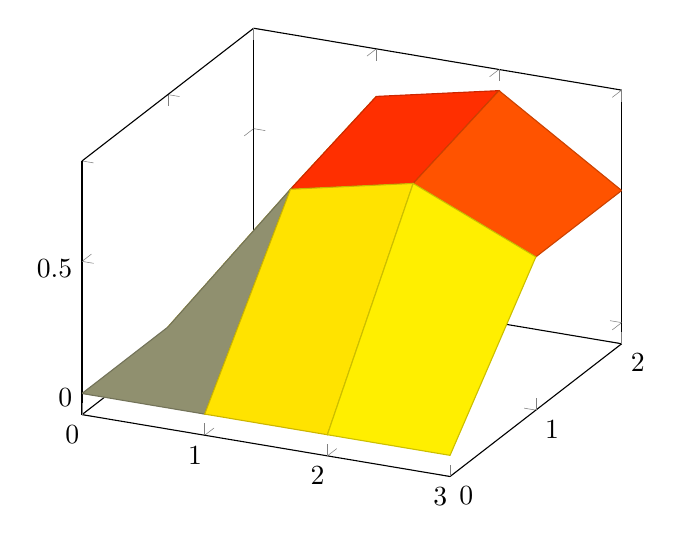
\begin{tikzpicture}
	\begin{axis}
		% this yields also a 3x4 matrix:
		\addplot3[surf,mesh/rows=3] coordinates {
			(0,0,0) (1,0,0)   (2,0,0)   (3,0,0)
			(0,1,0) (1,1,0.6) (2,1,0.7) (3,1,0.5)
			(0,2,0) (1,2,0.7) (2,2,0.8) (3,2,0.5)
		};
	\end{axis}
\end{tikzpicture}
\end{codeexample}

	It is enough to supply one of |mesh/rows| or |mesh/cols| -- the missing values will be determined automatically.
	
	If you provide one of |mesh/rows| or |mesh/cols|, any end--of--row marker seen inside of input files or coordinate streams will be ignored.

\end{pgfplotskeylist}

\begin{pgfplotskeylist}{mesh/scanline verbose=\mchoice{true,false} (initially false)}
	Provides debug messages in the \LaTeX\ output about end--of--scanline markers.

	The message will tell whether end--of--scanlines have been found and if they are the same.
\end{pgfplotskeylist}

\begin{pgfplotskey}{mesh/ordering=\mchoice{x varies,y varies,rowwise,colwise} (initially x varies)}
	Allows to configure the sequence in which matrices (meshes) are read from \verbpdfref{\addplot3 coordinates}, \verbpdfref{\addplot3 file} or \verbpdfref{\addplot3 table}.

	Here, \declaretext{x varies} means a sequence of points where $n$=|mesh/cols| successive points have the $y$ coordinate fixed. This is intuitive when you write down a function because $x$ is horizontal and $y$ vertical. Note that in matrix terminology, $x$ refers to \emph{column indices} whereas $y$ refers to \emph{row indices}. Thus, |x varies| is equivalent to \declaretext{rowwise} ordering in this sense. This is the initial configuration.
	
\long\def\temporarytest{\noexpand\par}
\begin{codeexample}[newline=\temporarytest]
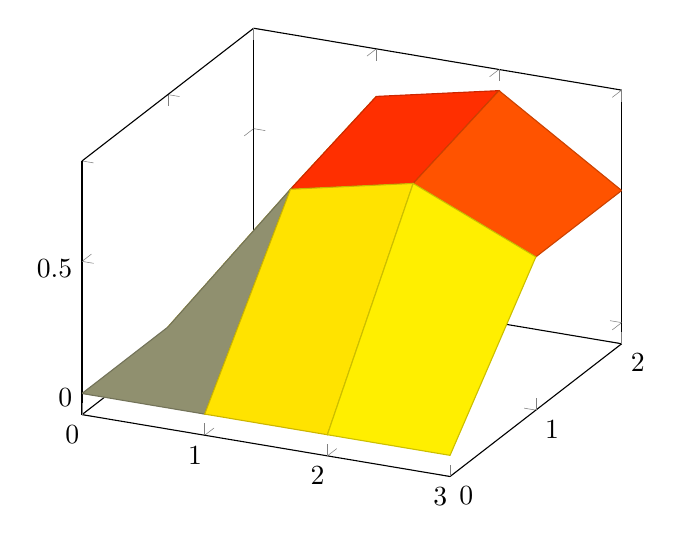
\begin{tikzpicture}
\begin{axis}[mesh/ordering=x varies]
	% this yields a 3x4 matrix in `x varies'
	% ordering:
	\addplot3[surf] coordinates {
		(0,0,0) (1,0,0)   (2,0,0)   (3,0,0)

		(0,1,0) (1,1,0.6) (2,1,0.7) (3,1,0.5)

		(0,2,0) (1,2,0.7) (2,2,0.8) (3,2,0.5)
	};
\end{axis}
\end{tikzpicture}
\end{codeexample}

	Consequently, |mesh/ordering=|\declaretext{y varies} provides points such that successive $m$=|mesh/rows| points form a column, i.e. the $x$ coordinate is fixed and the $y$ coordinate changes. In this sense, |y varies| is equivalent to \declaretext{colwise} ordering, it is actually a matrix transposition.
\long\def\temporarytest{\noexpand\par}
\begin{codeexample}[newline=\temporarytest]
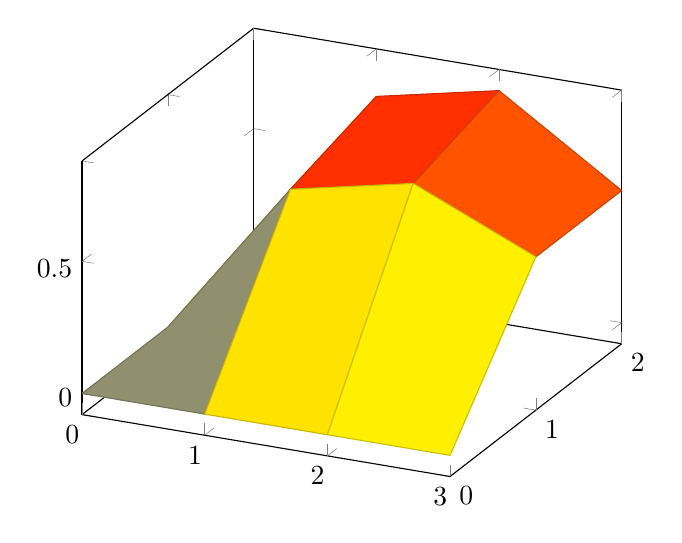
\begin{tikzpicture}
\begin{axis}[mesh/ordering=y varies]
	% this yields a 3x4 matrix in colwise ordering:
	\addplot3[surf] coordinates {
		(0,0,0) (0,1,0)   (0,2,0)

		(1,0,0) (1,1,0.6) (1,2,0.7)

		(2,0,0) (2,1,0.7) (2,2,0.8)

		(3,0,0) (3,1,0.5) (3,2,0.5)
	};
\end{axis}
\end{tikzpicture}
\end{codeexample}
	Again, note the subtle difference to the common matrix indexing where a column has the second index fixed. \PGFPlots\ refers to the way one would write down a function on a sheet of paper (this is consistent with how Matlab (tm) displays discrete functions with matrizes).

	Please note that |shader=interp| relies on low level shadings which need to be given in row wise ordering, so a (potentially expensive) transposition of the data matrix will be performed in this case. If possible, supply your data in row wise ordering for |shader=interp|.
\end{pgfplotskey}

\begin{addplot3operation}[]{\marg{math expression}}{}
\label{cmd:addplot3:expr}
	\pgfmanualpdflabel{\textbackslash addplot3 expression}{}%
	Expression plotting also works in the same way as for two dimensional plots. Now, however, a two dimensional mesh is sampled instead of a single line, which may depend on |x| and |y|.

	The method \verbpdfref{\addplot3} \marg{math expr} visualizes the function $f(x,y) = $\meta{math expr} where $ f \colon [x_1,x_2] \times [y_1,y_2] \to \R$. The interval $[x_1,x_2]$ is determined using the |domain| key, for example using |domain=0:1|. The interval $[y_1,y_2]$ is determined using the |y domain| key. If |y domain| is empty, $[y_1,y_2] = [x_1,x_2]$ will be assumed. If |y domain=0:0| (or any other interval of length zero), it is assumed that the plot does not depend on |y| (thus, it is a line plot).

	The number of samples in $x$ direction is set using the |samples| key. The number of samples in $y$ direction is set using the |samples y| key. If |samples y| is not set, the same value as for $x$ is used. If |samples y|$\le 1$, it is assumed that the plot does not depend on |y| (meaning it is a line plot).

\pgfplotsexpensiveexample
\begin{codeexample}[]
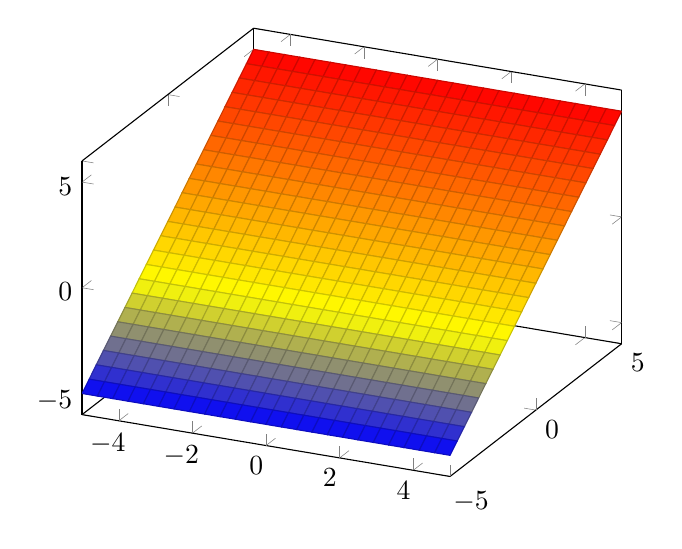
\begin{tikzpicture}
	\begin{axis}
		\addplot3[surf] {y};
	\end{axis}
\end{tikzpicture}
\end{codeexample}

\pgfplotsexpensiveexample
\begin{codeexample}[]
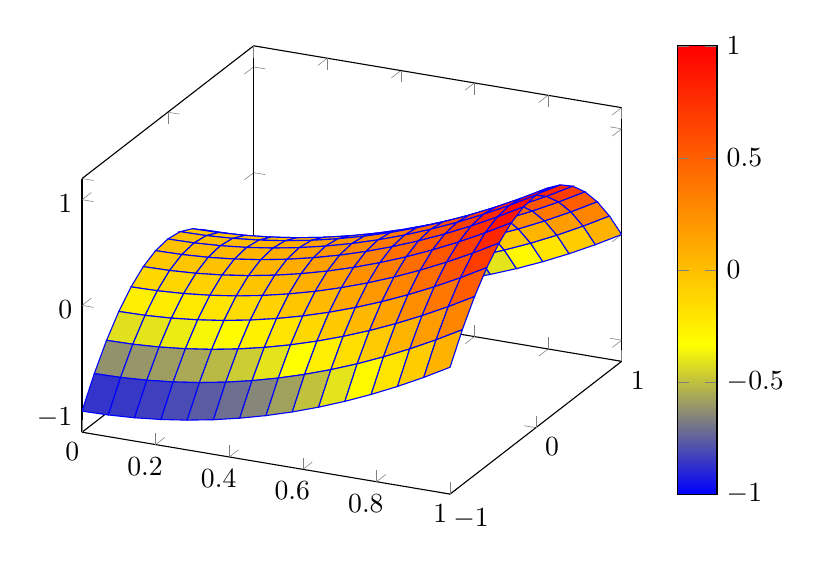
\begin{tikzpicture}
	\begin{axis}[colorbar]
		\addplot3
			[surf,faceted color=blue,
			 samples=15,
			 domain=0:1,y domain=-1:1]
			{x^2 - y^2};
	\end{axis}
\end{tikzpicture}
\end{codeexample}

	Expression plotting sets |mesh/rows| and |mesh/cols| automatically; these settings don't have any effect for expression plotting.
\end{addplot3operation}

\begin{addplot3operation}[]{expression}{\marg{math expr}}
	The syntax

	\verbpdfref{\addplot3} \marg{math expression}|;|

	as short-hand equivalent for

	\verbpdfref{\addplot3 expression} \marg{math expression}|;|
\end{addplot3operation}

\begin{addplot3operation}[]{(\meta{$x$ expression},\meta{$y$ expression},\meta{$z$ expression})}{}
	A variant of \verbpdfref{\addplot3 expression} which allows to provide different coordinate expressions for the $x$, $y$ and $z$ coordinates. This can be used to generate parameterized plots.

	Please note that |\addplot (x,y,x^2)| is equivalent to |\addplot expression {x^2}|.

	Note further that since the complete point expression is surrounded by round braces, round braces inside of \meta{$x$ expression}, \meta{$y$ expression} or \meta{$z$ expression} need to be treated specially. Surround the expressions (which contain round braces) with curly braces:

	|\addplot3 (|\marg{$x$ expr}|, |\marg{$y$ expr}|, |\marg{$z$ expr}|);|
\end{addplot3operation}

\subsubsection{Line Plots}

Three dimensional line plots are generated if the input source has no matrix structure. Line plots take the input coordinates and connect them in the order of appearance.

\begin{codeexample}[]
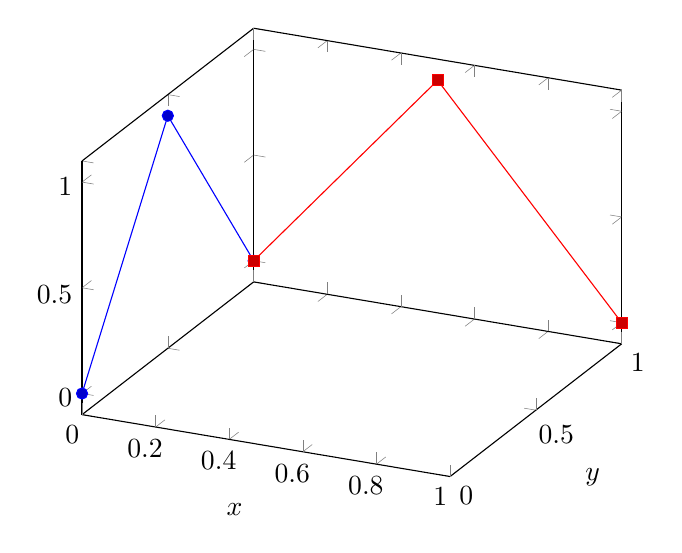
\begin{tikzpicture}
	\begin{axis}[xlabel=$x$,ylabel=$y$]
	\addplot3 coordinates {(0,0,0) (0,0.5,1) (0,1,0)};
	\addplot3 coordinates {(0,1,0) (0.5,1,1) (1,1,0)};
	\end{axis}
\end{tikzpicture}
\end{codeexample}
If there is no value for both, |mesh/rows| and |mesh/cols| or if one of them is |1|, \PGFPlots\ will draw a line plot. This is also the case if there is no end--of--scanline marker (empty line) in the input stream.

For \verbpdfref{\addplot3 expression}, this requires to set |samples y=0| to disable the generation of a mesh.
\begin{codeexample}[]
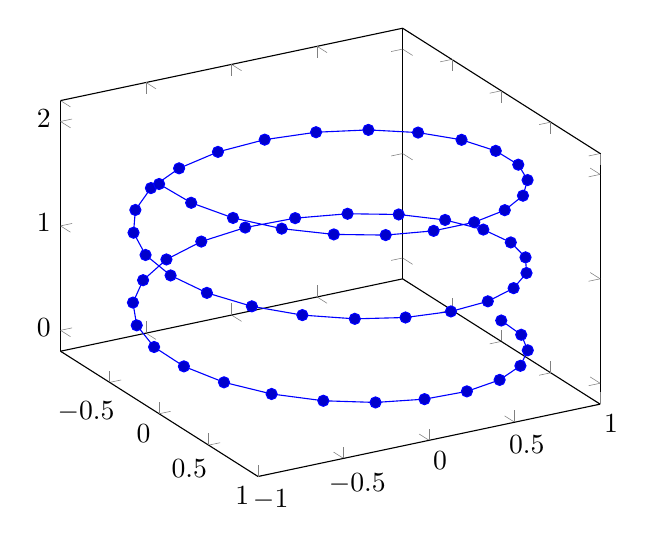
\begin{tikzpicture}
\begin{axis}[view={60}{30}]
\addplot3+[domain=0:5*pi,samples=60,samples y=0] 
	({sin(deg(x))},
	 {cos(deg(x))},
	 {2*x/(5*pi)});
\end{axis}
\end{tikzpicture}
\end{codeexample}

Three dimensional line plots will usually employ lines to connect points (i.e.\ the initial |sharp plot| handler of \Tikz). The |smooth| method of \Tikz\ might also prove be an option. Note that no piecewise constant plot, comb or bar plot handler is supported for three dimensional axes.

\subsubsection{Scatter Plots}

Three dimensional scatter plots have the same interface as for two dimensional scatter plots, so all examples of section~\ref{sec:pgfplots:scatter:2d} can be used for the three dimensional case as well. 
The key features are to use |only marks| and/or |scatter| as plot styles. 

We provide some more examples which are specific for the three dimensional case.

Our first example uses |only marks| to place the current plot |mark| at each input position:
\pgfplotsexpensiveexample
\begin{codeexample}[]
\begin{tikzpicture}
	\begin{axis}[
		xlabel=$x$,
		ylabel=$y$,
		zlabel={$f(x,y) = x\cdot y$},
		title=A Scatter Plot Example]
	% `pgfplotsexample4_grid.dat' contains a
	% large sequence of input points of the form
	% x_0   x_1     f(x)    
	% 0     0       0       
	% 0     0.03125 0       
	% 0     0.0625  0       
	% 0     0.09375 0       
	% 0     0.125   0       
	% 0     0.15625 0       
	\addplot3+[only marks] table
		{plotdata/pgfplotsexample4_grid.dat};
	\end{axis}
\end{tikzpicture}
\end{codeexample}

If we add the key |scatter|, the plot mark will also use the colors of the current |colormap|:
\pgfplotsexpensiveexample
\begin{codeexample}[]
\begin{tikzpicture}
	\begin{axis}[
		xlabel=$x$,
		ylabel=$y$,
		zlabel={$f(x,y) = x\cdot y$},
		title=A Scatter Plot Example]
	\addplot3+[only marks,scatter] table 
		{plotdata/pgfplotsexample4_grid.dat};
	\end{axis}
\end{tikzpicture}
\end{codeexample}

A more sophisticated example is to draw the approximated function as a |surf| plot (which requires matrix data) and the underlying grid (which is |scatter|ed data) somewhere into the same axis. We choose to place the $(x,y)$ grid points at $z=1.4$. Furthermore, we want the grid points to be colored according to the value of column |f(x)| in the input table:
\pgfplotsexpensiveexample
\begin{codeexample}[]
\begin{tikzpicture}
	\begin{axis}[
		3d box,
		zmax=1.4,
		colorbar,
		xlabel=$x$,
		ylabel=$y$,
		zlabel={$f(x,y) = x\cdot y$},
		title={Using Coordinate Filters to fix $z=1.4$}]
	% `pgfplotsexample4.dat' contains similar data as in 
	% `pgfplotsexample4_grid.dat', but it uses a uniform
	% matrix structure (same number of points in every scanline).
	% See examples above for extracts.
	\addplot3[surf,mesh/ordering=y varies] 
		table {plotdata/pgfplotsexample4.dat};
	\addplot3[scatter,scatter src=\thisrow{f(x)},only marks, z filter/.code={\def\pgfmathresult{1.4}}] 
		table {plotdata/pgfplotsexample4_grid.dat};
	\end{axis}
\end{tikzpicture}
\end{codeexample}
\noindent We used |z filter| to fix the $z$ coordinate to $1.4$. We could also have used the |table/z expr=1.4| feature
\begin{codeexample}[code only]
	\addplot3[scatter,scatter src=\thisrow{f(x)},only marks] 
		table[z expr=1.4] {plotdata/pgfplotsexample4_grid.dat};
\end{codeexample}
\noindent to get exactly the same effect. Choose whatever you like best. The |z filter| works for every coordinate input routine, the |z expr| feature is only available for |plot table|.


The following example uses |mark=cube*| and |z buffer=sort| to place boxes at each input coordinate. The color for each box is determined by |point meta={x+y+3}|. The remaining keys are just for pretty printing.
\pgfplotsexpensiveexample
\begin{codeexample}[]
\begin{tikzpicture}
\begin{axis}[
	view={120}{40},
	width=220pt,
	height=220pt,
	grid=major,
	z buffer=sort,
	xmin=-1,xmax=9,
	ymin=-1,ymax=9,
	zmin=-1,zmax=9,
	enlargelimits=upper,
	xtick={-1,1,...,19},
	ytick={-1,1,...,19},
	ztick={-1,1,...,19},
	xlabel={$l_1$},
	ylabel={$l_2$},
	zlabel={$l_3$},
	point meta={x+y+z+3},
	colormap={summap}{
		color=(black); color=(blue); 
		color=(black); color=(white) 
		color=(orange) color=(violet) 
		color=(red)
	},
	scatter/use mapped color={
		draw=mapped color,fill=mapped color!70},
	]
	% `pgfplots_scatter4.dat' contains a large sequence of
	% the form
	% l_0   l_1     l_2     
	% 1     6       -1      
	% -1    -1      -1      
	% 0     -1      -1      
	% -1    0       -1      
	% -1    -1      0       
	% 1     -1      -1      
	% 0     0       -1      
	% 0     -1      0       
	\addplot3[only marks,scatter,mark=cube*,mark size=7] 
		table {plotdata/pgfplots_scatterdata4.dat};

\end{axis}
\end{tikzpicture}
\end{codeexample}


\subsubsection{Mesh Plots}
\label{sec:2d:mesh}
\begin{plottype}[/pgfplots]{mesh}
	A mesh plot uses different colors for each mesh segment. Each mesh segment gets the same color. The color is determined using a ``color coordinate'' which is also called ``meta data'' throughout this document. It is the same data which is used for surface and scatter plots as well, see section~\ref{pgfplots:pointmeta}. In the initial configuration, the ``color coordinate'' is the $z$ axis (or the $y$ axis for two dimensional plots). This color coordinate is mapped linearly into the current color map to determine the color for each mesh segment. Thus, if the smallest occurring color data is, say, $-1$ and the largest is $42$, points with color data $-1$ will get the color at the lower end of the color map and points with color data $42$ the color of the upper end of the color map.

\pgfplotsexpensiveexample
\begin{codeexample}[]
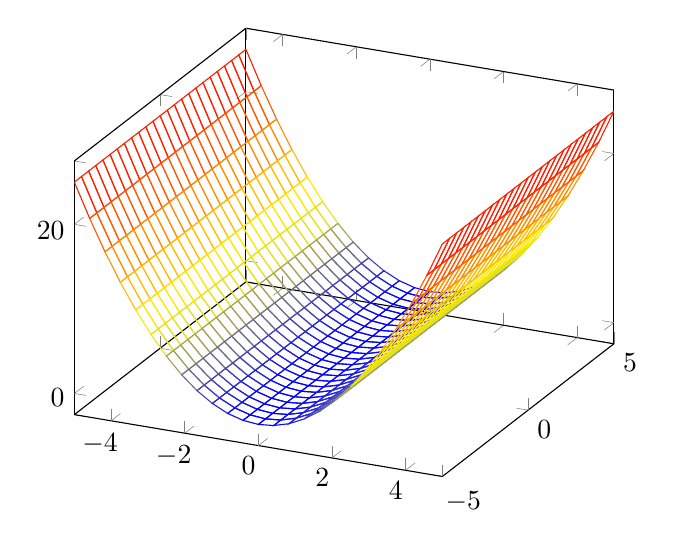
\begin{tikzpicture}
	\begin{axis}
		\addplot3[mesh] {x^2};
	\end{axis}
\end{tikzpicture}
\end{codeexample}

	A mesh plot can be combined with markers or with the |scatter| key which does also draw markers in different colors.

\pgfplotsexpensiveexample
\begin{codeexample}[]
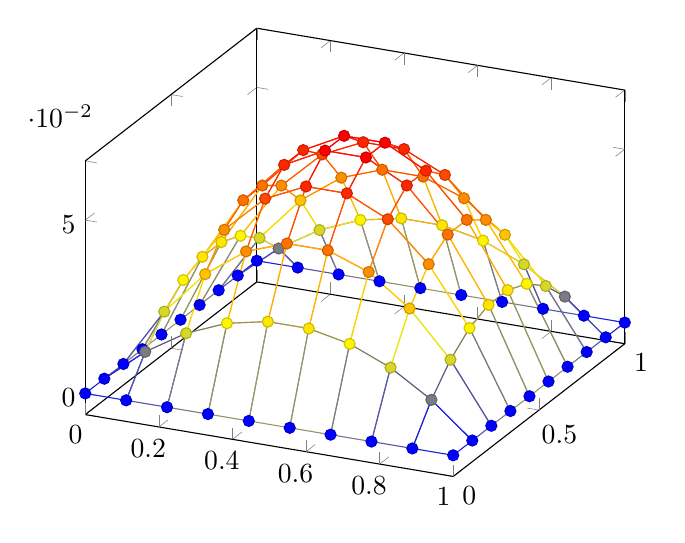
\begin{tikzpicture}
	\begin{axis}
	\addplot3+[mesh,scatter,samples=10,domain=0:1] 
		{x*(1-x)*y*(1-y)};
	\end{axis}
\end{tikzpicture}
\end{codeexample}

\pgfplotsexpensiveexample
\begin{codeexample}[]
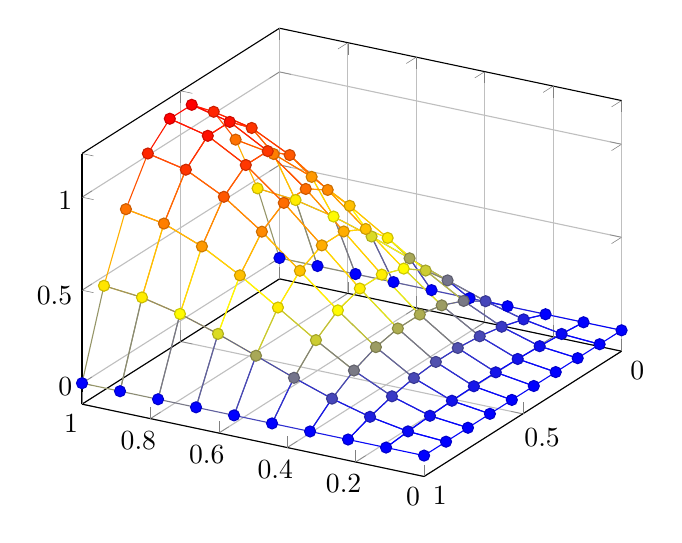
\begin{tikzpicture}
	\begin{axis}[grid=major,view={210}{30}]
	\addplot3+[mesh,scatter,samples=10,domain=0:1] 
		{5*x*sin(2*deg(x)) * y*(1-y)};
	\end{axis}
\end{tikzpicture}
\end{codeexample}

	\paragraph{Details:}
	\begin{itemize}
		\item 
	A mesh plot uses the same implementation as |shader=flat| to get one color for each single segment. Thus, if |shader=flat mean|, the color for a segment is determined using the \emph{mean} of the color data of adjacent vertices. If |shader=flat corner|, the color of a segment is the color of \emph{one} adjacent vertex.
		\item As soon as |mesh| is activated, |color=mapped color| is installed. This is \emph{necessary} unless one needs a different color -- but |mapped color| is the only color which reflects the color data.

		It is possible to use a different color using the |color=|\meta{color name} as for any other plot.

		\item It is easily possible to add |mark=|\meta{marker name} to mesh plots, |scatter| is also possible. Scatter plots will use the same color data as for the mesh.
	\end{itemize}

\pgfplotsexpensiveexample
\begin{codeexample}[]
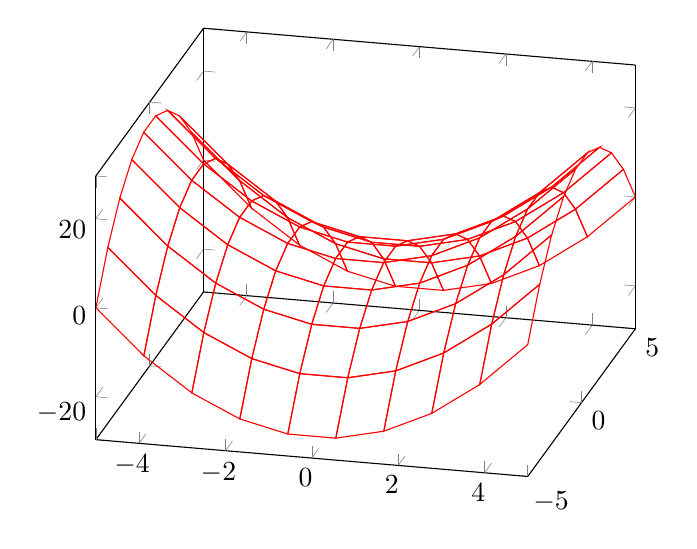
\begin{tikzpicture}
	\begin{axis}[view/az=14]
	\addplot3[mesh,draw=red,samples=10] {x^2-y^2};	
	\end{axis}
\end{tikzpicture}
\end{codeexample}
	
	Mesh plots use the |mesh legend| style to typeset legend images.
\end{plottype}

\begin{pgfplotskey}{mesh/check=\mchoice{false,warning,error} (initially error)}
	Allows to configure whether an error is generated if |mesh/rows| $\times$ |mesh/cols| does not equal the total number of coordinates.

	If you know exactly what you are doing, it may be useful to disable the check. If you are unsure, it is best to leave the initial setting.
\end{pgfplotskey}

\begin{pgfplotskey}{z buffer=\mchoice{default,none,auto,sort,reverse x seq,reverse y seq,reverse xy seq} (initially default)}
	This key allows to choose between different $z$ buffering strategies. A $z$ buffer determines which parts of an image should be drawn in front of other parts. Since both, the graphics packages \PGF\ and the final document format |.pdf| are inherently two dimensional, this work has to be done in \TeX. Currently, several (fast) heuristics can be used which work reasonably well for simple mesh- and surface plots. Furthermore, there is a (time consuming) sorting method which does also work if the fast heuristics fails.

	The $z$ buffering algorithms of \PGFPlots\ apply only to a single |\addplot| command. Different |\addplot| commands will be drawn on top of each other, in the order of appearance.

	The choice \declaretext{default} checks if we are currently working with a mesh or surface plot and uses |auto| in this case. If not, it sets |z buffer=none|.

	The choice \declaretext{none} disables $z$ buffering. This is also the case for two dimensional axes which don't need $z$ buffering.

	The choice \declaretext{auto} is the initial value for any mesh- or surface plot: it uses a very fast heuristics to decide how to realize $z$ buffering for mesh and surface plots. The idea is to reverse either the sequence of all $x$ coordinates, or those of all $y$ coordinates, or both. For regular meshes, this suffices to provide $z$ buffering. In other words: the choice |auto| will use one of the three reverse strategies |reverse |*| seq| (or none at all).

	The choice \declaretext{sort} can be used for scatter, line, mesh and surface plots. It really sorts according to the depth of each point (or mesh segment)\footnote{The choice \texttt{sort} is \emph{not} available for surface plots with \texttt{shader=interp} because the low level format doesn't support sorting.}. Sorting in \TeX\ uses a slow algorithm and may require a lot of memory (although it has the expected runtime asymptotics $\mathcal O(N \log N)$).

	The remaining choices apply only to mesh/surface plots and do nothing more then their name indicates: they reverse the coordinate sequences (using quasi linear runtime). They should only be used in conjunction by |z buffer=auto|.
\end{pgfplotskey}

\subsubsection{Surface Plots}
\label{sec:pgfplots:surfplots}
\begin{plottype}[/pgfplots]{surf}
	A surface plot visualizes a two dimensional, single patch using different fill colors for each patch segment. Each patch segment is a (pseudo) rectangle, that means input data is given in form of a data matrix as is discussed in the introductory section about three dimensional coordinates,~\ref{pgfplots:sec:threedim}.

\pgfplotsexpensiveexample
\begin{codeexample}[]
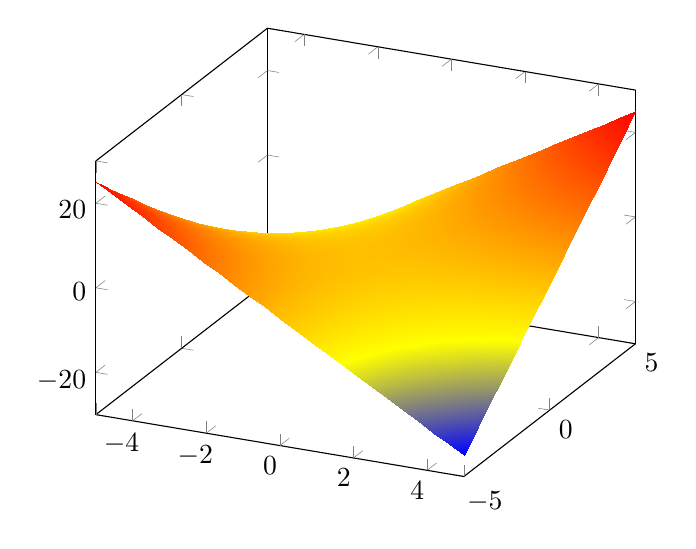
\begin{tikzpicture}
	\begin{axis}
		\addplot3[surf,shader=interp] {x*y};
	\end{axis}
\end{tikzpicture}
\end{codeexample}

	The simplest way to generate surface plots is to use the plot expression feature, but -- as discussed in section~\ref{pgfplots:sec:threedim} -- other input methods like \verbpdfref{\addplot3 table} or \verbpdfref{\addplot3 coordinates} are also possible. 

	The appearance can be configured using |colormap|s, the value of the |shader|, |faceted color| keys and the current |color| and/or |draw| / |fill| color. As for |mesh| plots, the special |color=mapped color| is installed for the faces. The stroking color for faceted plots can be set with |faceted color| (see below for details).

\pgfplotsexpensiveexample
\begin{codeexample}[]
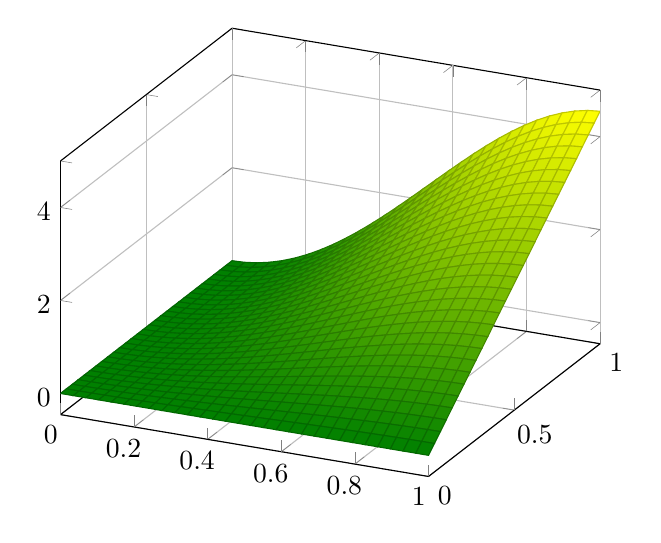
\begin{tikzpicture}
	\begin{axis}[
		grid=major,
		colormap/greenyellow]
	\addplot3[surf,samples=30,domain=0:1] 
		{5*x*sin(2*deg(x)) * y};
	\end{axis}
\end{tikzpicture}
\end{codeexample}

\pgfplotsexpensiveexample
\begin{codeexample}[]
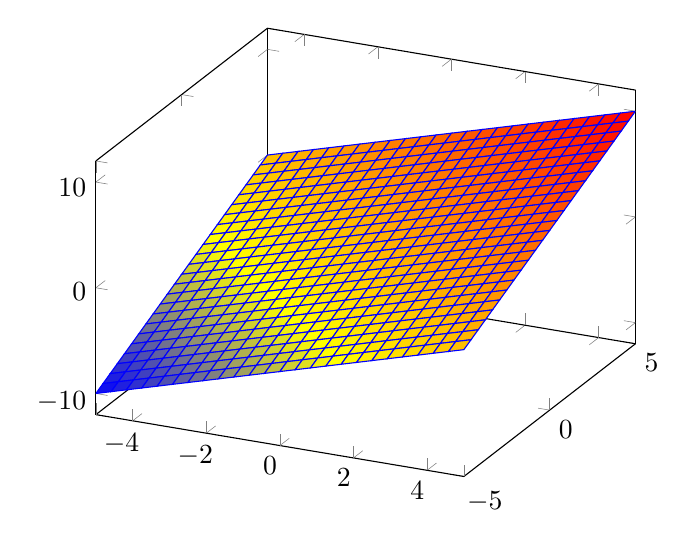
\begin{tikzpicture}
	\begin{axis}
		\addplot3[surf,faceted color=blue] {x+y};
	\end{axis}
\end{tikzpicture}
\end{codeexample}

\pgfplotsexpensiveexample
\begin{codeexample}[]
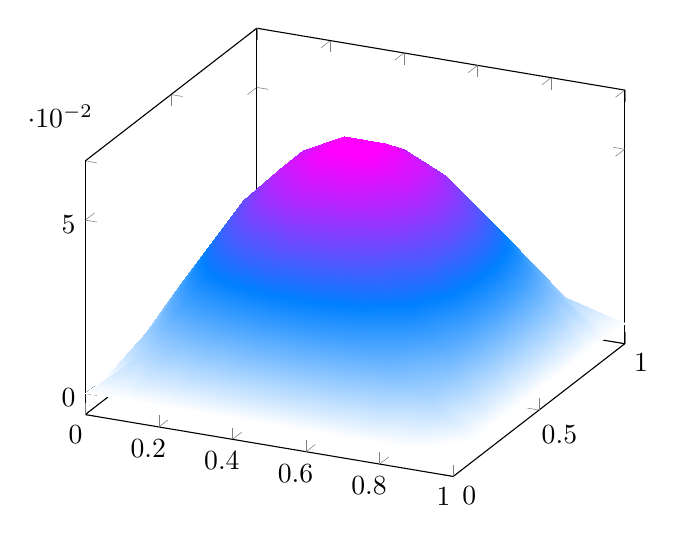
\begin{tikzpicture}
	\begin{axis}[colormap/cool]
	\addplot3[surf,samples=10,domain=0:1,
		shader=interp] 
		{x*(1-x)*y*(1-y)};
	\end{axis}
\end{tikzpicture}
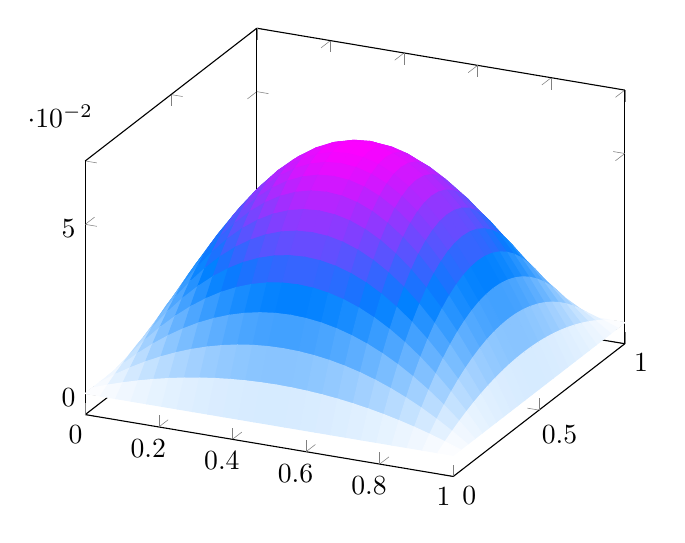
\begin{tikzpicture}
	\begin{axis}[colormap/cool]
	\addplot3[surf,samples=25,domain=0:1,
		shader=flat] 
		{x*(1-x)*y*(1-y)};
	\end{axis}
\end{tikzpicture}
\end{codeexample}

\pgfplotsexpensiveexample
\begin{codeexample}[]
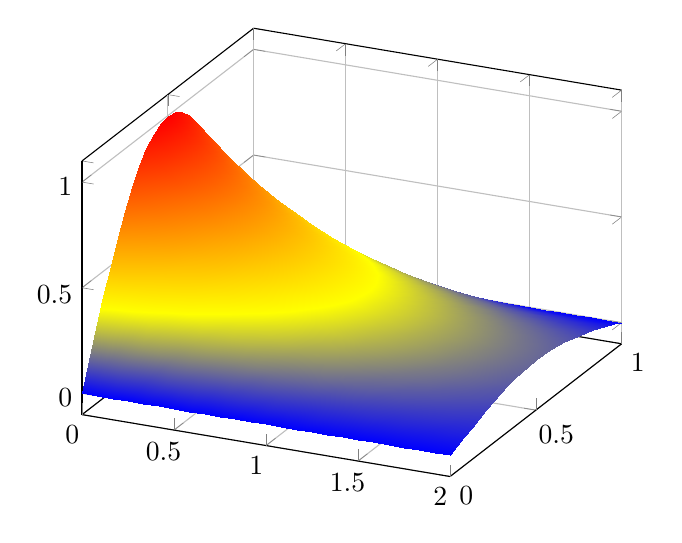
\begin{tikzpicture}
	\begin{axis}[grid=major]
		\addplot3[surf,shader=interp,
			samples=25,domain=0:2,y domain=0:1] 
			{exp(-x) * sin(pi*deg(y))};
	\end{axis}
\end{tikzpicture}
\end{codeexample}

\pgfplotsexpensiveexample
\begin{codeexample}[]
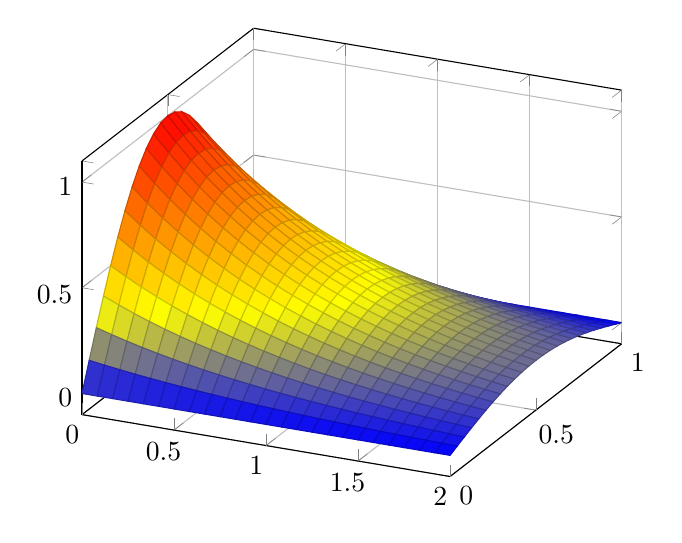
\begin{tikzpicture}
	\begin{axis}[grid=major]
		\addplot3[surf,shader=faceted,
			samples=25,domain=0:2,y domain=0:1] 
			{exp(-x) * sin(pi*deg(y))};
	\end{axis}
\end{tikzpicture}
\end{codeexample}

	Details about the shading algorithm are provided below in the documentation of |shader|.

	Surface plots use the |mesh legend| style to create legend images.
\end{plottype}

\begin{pgfplotskey}{shader=\mchoice{flat,interp,faceted,flat corner,flat mean} (initially faceted)}
	Configures the shader used for surface plots. The shader determines how the color data available at each single vertex is used to fill the surface patch.

	The simplest choice is to use one fill color for each segment, the choice |flat|.

\pgfplotsexpensiveexample
\begin{codeexample}[]
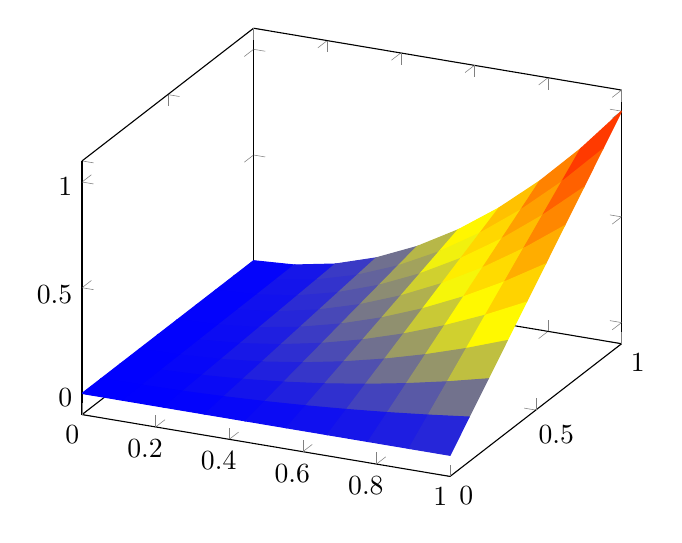
\begin{tikzpicture}
	\begin{axis}
	\addplot3[surf,shader=flat,
		samples=10,domain=0:1] 
		{x^2*y};
	\end{axis}
\end{tikzpicture}
\end{codeexample}

	\noindent The |flat| shader provides full support of |z buffer|ing, that means it does also support the choice |z buffer=sort|. There are (currently) two possibilities to determine the single color for every segment:
	\begin{description}
		\item[\declaretext{flat corner}] Uses the color data of one vertex to color the segment. It is not defined which vertex is used here\footnote{\PGFPlots\ just uses the last vertex encountered in its internal processings -- but after any $z$ buffer re-orderings.}.

		\item[\declaretext{flat mean}] Uses the mean of all four color data values as segment color. This is the initial value as it provides symmetric colors for symmetric functions.
	\end{description}
	The choice |flat| is actually the same as |flat mean|. Please note that |shader=flat mean| and |shader=flat corner| also influence mesh plots -- the choices determine the mesh segment color.

	Another choice is |shader=|\declareandlabel{interp} which uses Goraud shading (smooth linear interpolation of two triangles approximating rectangles) to fill the segments. 

\pgfplotsexpensiveexample
\begin{codeexample}[]
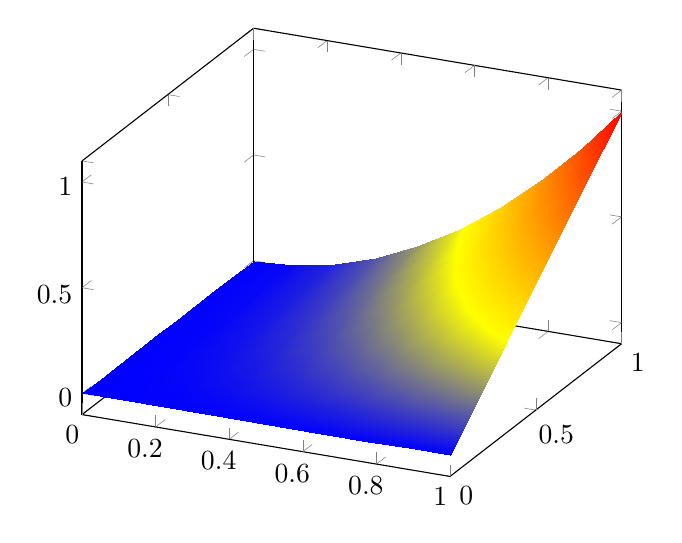
\begin{tikzpicture}
	\begin{axis}
	\addplot3[surf,shader=interp,
		samples=10,domain=0:1] 
		{x^2*y};
	\end{axis}
\end{tikzpicture}
\end{codeexample}

	The |shader=interp| setting requires a special low--level shading implementation which is currently (only) available for the postscript driver \declaretext{pgfsys-dvips.def} and the |pdflatex| driver \declaretext{pgfsys-pdftex.def}. For other drivers, the choice |shader=interp| will result in a warning and is equivalent to |shader=flat mean|. 
	


	Finally, the choice |shader=faceted| uses a constant fill color for every mesh segment (as for |flat|) and the value of the key |/pgfplots/faceted color| to draw the connecting mesh elements:
\pgfplotsexpensiveexample
\begin{codeexample}[]
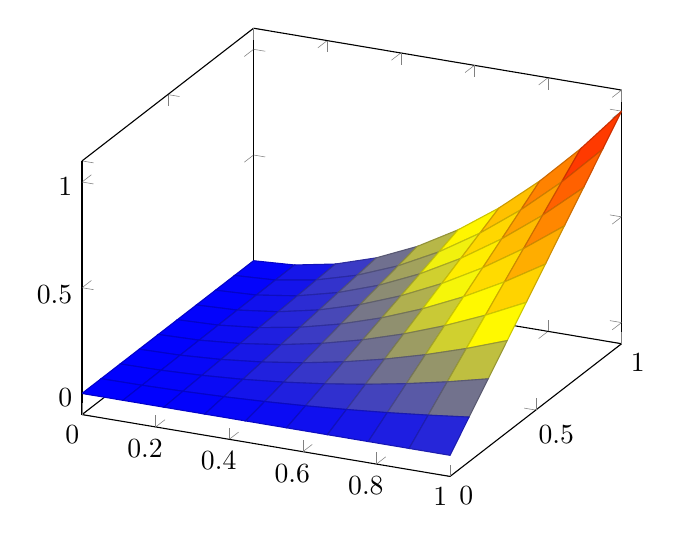
\begin{tikzpicture}
	\begin{axis}
	\addplot3[surf,shader=faceted,
		samples=10,domain=0:1] 
		{x^2*y};
	\end{axis}
\end{tikzpicture}
\end{codeexample}


	\paragraph{Details:}
	\begin{itemize}
		\item The choice |shader=faceted| is the same as |shader=flat| -- except that it uses a special draw color.
		
		So, |shader=faceted| has the same effect as 
		
		|shader=flat,draw=\pgfkeysvalueof{/pgfplots/faceted color}|.

		\item The |flat| shader uses the current |draw| and |fill| colors. They are set with |color=mapped color| and can be overruled with |draw=|\meta{draw color} and |fill=|\meta{fill color}. The |mapped color| always contains the color of the color map. 
		
		\item The |interp| shader does not support mesh colors and it uses the current color map in any case (it simply ignores the values of |draw| and |fill|).

		\item You easily add |mark=|\meta{plot mark} to mesh and/or surface plots or even colored plot marks with |scatter|. The scatter plot feature will use the same color data as for the surface.

		But: Markers and surfaces do not share the same depth information. They are drawn on top of each other.

		\item For surface plots with lots of points, |shader=interp| produces smaller |pdf| documents, requires less compilation time in \TeX\ and requires less time to display in Acrobat Reader.

		\item The postscript driver did not work when I tried to write hex encoded 32 bit binary coordinates into the shading. So, the postscript driver \emph{truncates} coordinates to 24 bit -- which might result in a loss of precision (the truncation is not very intelligent). See the |surf shading/precision| key for details. To improve compatibility, this 24 bit truncation algorithm is enabled by default.
	\end{itemize}

\pgfplotsexpensiveexample
\begin{codeexample}[]
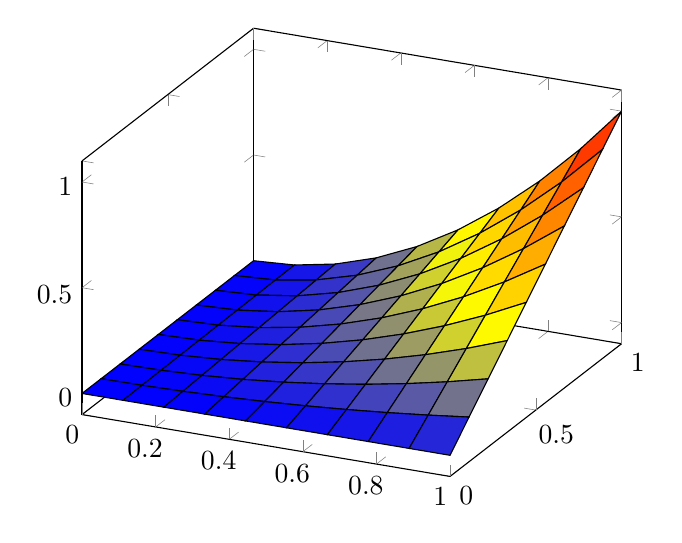
\begin{tikzpicture}
	\begin{axis}
	\addplot3[surf,shader=flat,
		draw=black,
		samples=10,domain=0:1] 
		{x^2*y};
	\end{axis}
\end{tikzpicture}
\end{codeexample}

\pgfplotsexpensiveexample
\begin{codeexample}[]
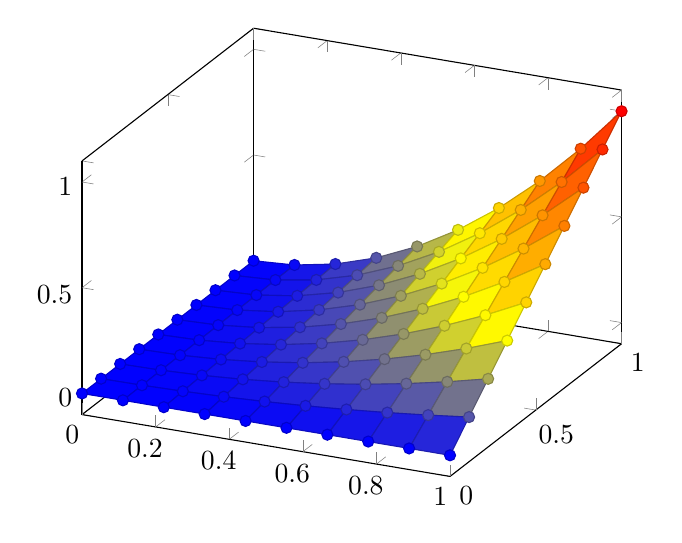
\begin{tikzpicture}
	\begin{axis}
	\addplot3[surf,shader=faceted,
		scatter,mark=*,
		samples=10,domain=0:1] 
		{x^2*y};
	\end{axis}
\end{tikzpicture}
\end{codeexample}
\end{pgfplotskey}

\begin{pgfplotskey}{faceted color=\marg{color name} (initially mapped color!80!black)}
	Defines the color to be used for meshes of faceted surface plots.
\end{pgfplotskey}

\begin{pgfplotskey}{surf shading/precision=\mchoice{pdf,postscript,ps} (initially postscript)}
	A key to configure how the low level driver for |shader=interp| writes its data. The choice |pdf| uses 32 bit binary coordinates (which is lossless). The resulting |.pdf| files appear to be correct, but they can't be converted to postscript -- the converter software always complaints about an error. 

	The choice |postscript| (or, in short, |ps|) uses 24 bit truncated binary coordinates. This results in both, readable |.ps| and |.pdf| files. However, the truncation is lossy.

	If anyone has ideas how to fix this problem: let me know. As far as I know, postscript should accept 32 bit coordinates, so it might be a mistake in the shading driver.
\end{pgfplotskey}

\subsubsection{Parameterized Plots}
Parameterized plots use the same plot types as documented in the preceding sections: both, mesh and surface plots are actually special parameterized plots where $x$ and $y$ are on cartesian grid points.

Parameterized plots just need a special way to provide the coordinates:

\pgfplotsexpensiveexample
\begin{codeexample}[]
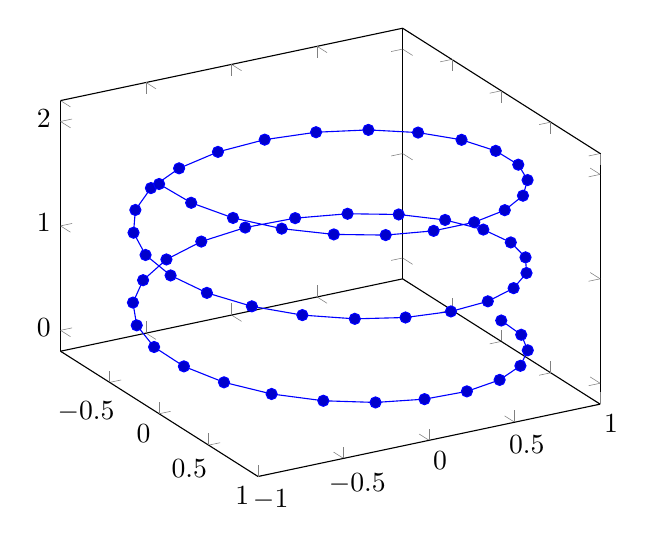
\begin{tikzpicture}
	\begin{axis}[view={60}{30}]
	\addplot3+[domain=0:5*pi,samples=60,samples y=0] 
		({sin(deg(x))},
		 {cos(deg(x))},
		 {2*x/(5*pi)});
	\end{axis}
\end{tikzpicture}
\end{codeexample}
\noindent The preceding example uses |samples y=0| to indicate that a line shall be samples instead of a matrix. The curly braces are necessary because \TeX\ can't nest round braces. The single expressions here are used to parameterize the helix.

Another example follows. Note that |z buffer=sort| is a necessary method here.

\pgfplotsexpensiveexample
\begin{codeexample}[]
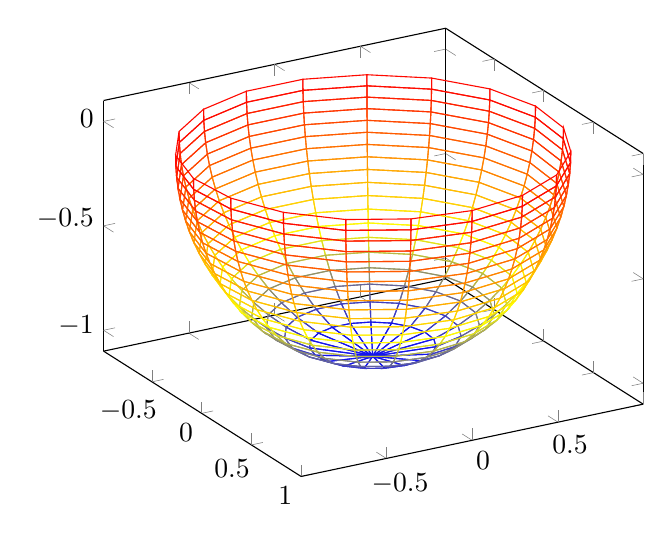
\begin{tikzpicture}
\begin{axis}[view={60}{30}]
	\addplot3[mesh,z buffer=sort,
		samples=20,domain=-1:0,y domain=0:2*pi]
		({sqrt(1-x^2) * cos(deg(y))},
		 {sqrt( 1-x^2 ) * sin(deg(y))},
		 x);
\end{axis}
\end{tikzpicture}
\end{codeexample}

\pgfplotsexpensiveexample
\begin{codeexample}[]
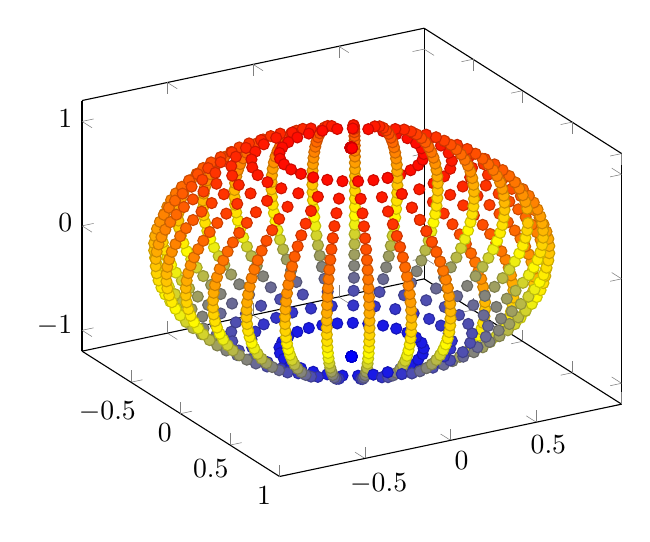
\begin{tikzpicture}
\begin{axis}[view={60}{30}]
	\addplot3[mesh,z buffer=sort,
		scatter,only marks,scatter src=z,
		samples=30,domain=-1:1,y domain=0:2*pi]
		({sqrt(1-x^2) * cos(deg(y))},
		 {sqrt( 1-x^2 ) * sin(deg(y))},
		 x);
\end{axis}
\end{tikzpicture}
\end{codeexample}

\pgfplotsexpensiveexample
\begin{codeexample}[]
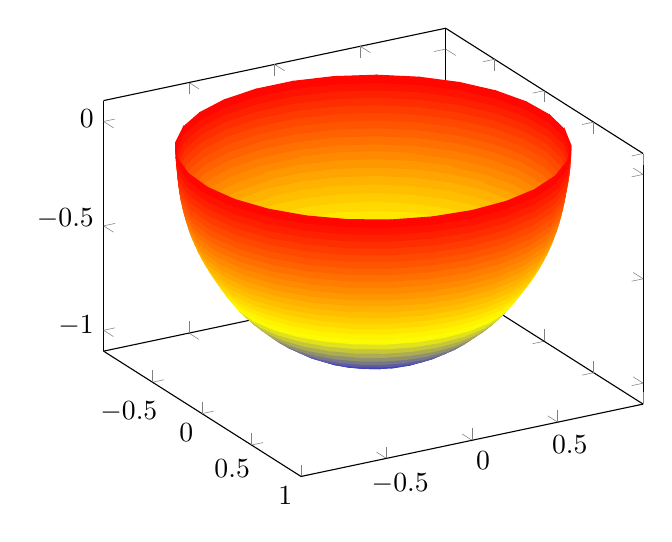
\begin{tikzpicture}
\begin{axis}[view={60}{30}]
	\addplot3[surf,shader=flat,z buffer=sort,
		samples=30,domain=-1:0,y domain=0:2*pi]
		({sqrt(1-x^2) * cos(deg(y))},
		 {sqrt( 1-x^2 ) * sin(deg(y))},
		 x);
\end{axis}
\end{tikzpicture}
\end{codeexample}

\subsubsection{About 3D Const Plots and 3D Bar Plots}
There are currently \emph{no} equivalents of |const plot| and its variants or the bar plot types like |ybar| for three dimensional axes, sorry.

